\chapter{ch3半导体中载流子的统计分布}
\section{能量状态密度}
\begin{definition}{状态密度}
    能带中，能量E附近单位能量间隔内量子态数即为状态密度，
    \[
    g(E) = \frac{dZ}{dE}
    \]
    其中$dZ$是能量$E$到$E+dE$之间的量子态数。
\end{definition}

\begin{theorem}{电子与空穴的状态密度}
    \begin{itemize}
        \item 电子状态密度可以表示为 \[g_c(E)=\frac{V}{2\pi^2}\frac{(2m_{n}^{*})^{3/2}}{\hbar^3}[E-E_c]^{1/2}\]
        \item 空穴状态密度可以表示为 \[g_v(E)=\frac{V}{2\pi^2}\frac{(2m_{p}^{*})^{3/2}}{\hbar^3}[E_v-E]^{1/2}\]
    \end{itemize}
    值得注意的是，若等能面是球面（比如AsGa），$m_{n}^{*}$和$m_{p}^{*}$直接等于电子/空穴的质量；若等能面是椭球体（Si和Ge），则需要考虑轻重电子/空穴，此时$m_{n}^{*}$和$m_{p}^{*}$就是轻重电子/空穴质量的等效表达式。
    
\end{theorem}


\begin{problem}
    计算能量在$E=E_c$到
    $E=E_c+100\left(\dfrac{\pi^2\hbar^2}{2m_n^*L^2}\right)$
    之间单位体积中的量子态数，其中$L$为立方体样品的边长。

    \textbf{解析：}采用上述导带状态密度（已计入自旋简并），令
    $\Delta E=100\pi^2\hbar^2/(2m_n^*L^2)$。
    对单位体积状态密度$g_c(E)/V$积分，得
    \begin{align*}
        \frac{\Delta Z}{V}
        &=\int_{E_c}^{E_c+\Delta E}\frac{g_c(E)}{V}\,\mathrm{d}E\\
        &=\frac{(2m_n^*)^{3/2}}{2\pi^2\hbar^3}
        \int_0^{\Delta E}\varepsilon^{1/2}\,\mathrm{d}\varepsilon\\
        &=\frac{(2m_n^*)^{3/2}}{3\pi^2\hbar^3}(\Delta E)^{3/2}\\
        &=\boxed{\frac{1000\pi}{3L^3}}.
    \end{align*}
\end{problem}

\section{费米能级}
\begin{definition}{费米能级与费米分布}
    费米分布以量子理论为基础，\textbf{能量量子化，不连续，满足泡利不相容原理}，据此可以推导出电子按能量的大小有一定的统计分布规律$f(E)$
    \[
    f(E) = \frac{1}{1+exp(\frac{E-\textcolor{red}{E_F}}{k_0 T})}
    \]
    其中$E_F$表示费米能级。半导体系统需要极高的掺杂（$>10^18cm^{-3}$）才需要考虑泡利不相容，满足条件的系统称为\textbf{简并系统}。
\end{definition}

\begin{remark}
    \begin{itemize}
        \item 费米能级的高低和\textbf{半导体材料的导电类型、杂质含量、温度、能量零点}有关。
        \item 热平衡时，系统有统一的费米能级。
        \item 费米能级对应的量子态中恰好有一半被电子填充，更低的能级被电子填充过半，更高的则少于一半。
    \end{itemize}
    
\end{remark}

\begin{definition}{玻尔兹曼分布}
    玻尔兹曼分布以经典理论为基础，\textbf{能量可以取任意值，是连续的，不需要考虑泡利不相容原理}。\textbf{\textcolor{red}{当系统的掺杂浓度较低的时候，费米分布退化为玻尔兹曼分布}}：
    \[
    f(E)=exp(-\frac{E-E_F}{k_0T})
    \]
    满足条件的系统称为\textbf{非简并系统}。
\end{definition}

\section{载流子的统计分布}
在一般情况下，半导体系统中并没有很高的掺杂，费米能级$E_F$位于禁带内，而且与导带底和价带顶的距离远大于$k_0T$，此时导带底电子和价带顶空穴满足玻尔兹曼分布。
此时，根据积分$N=\int^{E'}{E}f(E)g(E)dE$可以求得电子和空穴的浓度。

\begin{theorem}{非简并半导体载流子分布}
    电子分布：
    \[n_0=N_c exp(-\frac{E_c-E_F}{k_0 T})\]
    其中
    \[N_c=2 \frac{(2\pi m_n^{*}k_0T)^{3/2}}{h^3}\]
    空穴分布：
    \[n_0=N_v exp(-\frac{E_F-E_v}{k_0 T})\]
    其中
    \[N_c=2 \frac{(2\pi m_p^{*}k_0T)^{3/2}}{h^3}\]

\end{theorem}

\begin{theorem}{载流子乘积推论}
    一定的半导体，如果温度一定，则乘积一定。与费米能级无关，与杂质浓度无关。
    \[n_0p_0 = N_cN_vexp(-\frac{E_c-E_v}{k_0T})=N_cN_vexp(-\frac{E_g}{k_0T})\]
    \textbf{\textcolor{red}{注意此推论只适用于简并系统，在非简并系统中不成立！}}
\end{theorem}

\section{本征半导体的载流子浓度}
\begin{theorem}{本征半导体的费米能级}
    本征半导体具有$n_0=p_0$的性质，据此可以得出：
    \[E_i=\frac{E_c+E_v}{2}+\frac{k_0T}{2}ln\frac{N_v}{N_c}\]

\end{theorem}

\begin{theorem}{推论}
    由：
    \[n_i=p_i=N_cexp(-\frac{E_c-E_i}{k_0T})=N_vexp(-\frac{E_i-E_v}{k_0T})\]
    可以将杂质半导体的载流子浓度用$E_i$（而非$E_c$或$E_v$）表示：
    \[n_0=n_iexp(-\frac{E_i-E_F}{k_0T})\]
    \[p_0=n_iexp(-\frac{E_F-E_i}{k_0T})\]
\end{theorem}

\begin{problem}
    \textbf{所用常数与单位：}
    \[
    \begin{aligned}
        h&=6.62607015\times10^{-34}\ \mathrm{J\cdot s},\\
        k_0&=1.380649\times10^{-23}\ \mathrm{J\cdot K^{-1}}
        =8.617333262\times10^{-5}\ \mathrm{eV\cdot K^{-1}},\\
        m_0&=9.1093837\times10^{-31}\ \mathrm{kg},\qquad g_D=2.
    \end{aligned}
    \]

    \textbf{题面：}
    \begin{enumerate}
        \item 室温下，锗的有效态密度为
        $N_c=1.05\times10^{19}\ \mathrm{cm}^{-3}$、
        $N_v=3.9\times10^{18}\ \mathrm{cm}^{-3}$。
        求载流子有效质量$m_n^*,m_p^*$，并计算$77\ \mathrm{K}$时的$N_c,N_v$。
        已知$300\ \mathrm{K}$时$E_g=0.67\ \mathrm{eV}$，
        $77\ \mathrm{K}$时$E_g=0.76\ \mathrm{eV}$，求两个温度下的本征载流子浓度。
        \item $77\ \mathrm{K}$时，锗的电子浓度为
        $n_0=10^{17}\ \mathrm{cm}^{-3}$，受主浓度为零，
        且$E_c-E_D=0.01\ \mathrm{eV}$，求施主浓度$N_D$。
    \end{enumerate}

    \textbf{解析：}采用非简并近似，并假定态密度有效质量不随温度变化。

    \textbf{（1）有效质量、有效态密度及本征浓度。}
    由$N=2(2\pi m^*k_0T/h^2)^{3/2}$反解得
    \[
    m^*=\frac{h^2}{2\pi k_0T}\left(\frac{N}{2}\right)^{2/3}.
    \]
    计算质量时，$N$须换成$\mathrm{m}^{-3}$，$k_0$采用焦耳单位。
    \begin{center}
        \begin{tabular}{c c c c}
            \hline
            载流子 & $N(300\ \mathrm{K})\ (\mathrm{m}^{-3})$ & $m^*\ (\mathrm{kg})$ & $m^*/m_0$ \\
            \hline
            电子 & $1.05\times10^{25}$ & $5.10\times10^{-31}$ & $0.559$ \\
            空穴 & $3.90\times10^{24}$ & $2.63\times10^{-31}$ & $0.289$ \\
            \hline
        \end{tabular}
    \end{center}
    这里求得的是\textbf{态密度有效质量}。利用
    \[
    N_{c,v}(T)=N_{c,v}(300)\left(\frac{T}{300}\right)^{3/2},
    \qquad
    n_i=\sqrt{N_cN_v}\exp\!\left(-\frac{E_g}{2k_0T}\right),
    \]
    其中$(77/300)^{3/2}=0.1300$；指数中的能量均取$\mathrm{eV}$。
    两个温度下的重复计算汇总如下，所有浓度单位均为$\mathrm{cm}^{-3}$。
    \begin{center}
        \begin{tabular}{c c c c}
            \hline
            物理量 & 计算式 & $300\ \mathrm{K}$ & $77\ \mathrm{K}$ \\
            \hline
            $N_c$ & $1.05\times10^{19}(T/300)^{3/2}$ & $1.05\times10^{19}$ & $1.37\times10^{18}$ \\
            $N_v$ & $3.90\times10^{18}(T/300)^{3/2}$ & $3.90\times10^{18}$ & $5.07\times10^{17}$ \\
            $E_g\ (\mathrm{eV})$ & 题给 & $0.67$ & $0.76$ \\
            $k_0T\ (\mathrm{eV})$ & $8.617333262\times10^{-5}T$ & $0.02585$ & $0.006635$ \\
            $n_i$ & $\sqrt{N_cN_v}\exp[-E_g/(2k_0T)]$ & $1.51\times10^{13}$ & $1.12\times10^{-7}$ \\
            \hline
        \end{tabular}
    \end{center}

    \textbf{（2）施主浓度。}
    在$77\ \mathrm{K}$下，$p_0=n_i^2/n_0\ll n_0$，且$N_A=0$，
    电中性条件给出$n_D^+=n_0-p_0\simeq n_0$。
    由电子浓度和施主电离公式，
    \begin{align*}
        E_c-E_F&=k_0T\ln\frac{N_c}{n_0}=0.01734\ \mathrm{eV},\\
        E_F-E_D&=(E_c-E_D)-(E_c-E_F)=-0.007345\ \mathrm{eV},\\
        n_D^+&=\frac{N_D}{1+2\exp[(E_F-E_D)/(k_0T)]}.
    \end{align*}
    因此
    \begin{align*}
        N_D&\simeq n_0\left[1+2\exp\!\left(\frac{E_F-E_D}{k_0T}\right)\right]\\
        &=10^{17}\left[1+2\exp\!\left(\frac{-0.007345}{0.006635}\right)\right]\\
        &\boxed{\simeq1.66\times10^{17}\ \mathrm{cm}^{-3}}.
    \end{align*}
    施主电离率约为$n_D^+/N_D\simeq60.2\%$，故不能直接令$N_D=n_0$。
\end{problem}

\section{杂质半导体的载流子浓度}

\begin{theorem}{杂质能级的占据概率与电离浓度}
    杂质能级最多容纳一个电子，需计入基态简并度，不能直接用标准费米分布描述。
    施主被电子占据、受主被空穴占据的概率分别为
    \[
    f_D=\frac{1}{1+\dfrac{1}{g_D}\exp\!\left(\dfrac{E_D-E_F}{k_0T}\right)},
    \qquad
    f_A=\frac{1}{1+\dfrac{1}{g_A}\exp\!\left(\dfrac{E_F-E_A}{k_0T}\right)}.
    \]
    其中$E_D,E_A$为施主、受主能级，$N_D,N_A$为对应杂质浓度；
    对硅、锗、砷化镓，通常取$g_D=2$、$g_A=4$。

    未电离杂质呈电中性，其能级上的电子、空穴浓度分别为
    \[
    n_D=N_Df_D=\frac{N_D}{1+\dfrac{1}{2}\exp\!\left(\dfrac{E_D-E_F}{k_0T}\right)},
    \qquad
    p_A=N_Af_A=\frac{N_A}{1+\dfrac{1}{4}\exp\!\left(\dfrac{E_F-E_A}{k_0T}\right)}.
    \]
    电离施主带正电，电离受主带负电，其浓度分别为
    \begin{align*}
        n_D^+&=N_D-n_D
        =\frac{N_D}{1+2\exp\!\left(\dfrac{E_F-E_D}{k_0T}\right)},\\
        p_A^-&=N_A-p_A
        =\frac{N_A}{1+4\exp\!\left(\dfrac{E_A-E_F}{k_0T}\right)}.
    \end{align*}
\end{theorem}

\begin{theorem}{不同温度区间的半导体的费米能级和杂质电离程度}
    以下适用于非简并、单一施主或受主掺杂的半导体，取$g_D=2$、$g_A=4$。
    随温度升高，依次经历以下五个区间。

    \textbf{一、杂质电离区：}本征激发可忽略，电中性条件为
    $n_0\simeq n_D^+$（N型）或$p_0\simeq p_A^-$（P型）。
    \begin{enumerate}
        \item \textbf{低温弱电离区：}杂质仅少量电离，
        \[
        n_D^+\simeq\frac{N_D}{2}\exp\!\left(\frac{E_D-E_F}{k_0T}\right),
        \qquad
        p_A^-\simeq\frac{N_A}{4}\exp\!\left(\frac{E_F-E_A}{k_0T}\right).
        \]
        结合载流子的玻尔兹曼分布，得
        \begin{align*}
            \text{N型：}\quad E_F&=\frac{E_c+E_D}{2}+\frac{k_0T}{2}\ln\frac{N_D}{2N_c},\\
            n_0&\simeq\sqrt{\frac{N_DN_c}{2}}\exp\!\left(-\frac{E_c-E_D}{2k_0T}\right);\\
            \text{P型：}\quad E_F&=\frac{E_v+E_A}{2}-\frac{k_0T}{2}\ln\frac{N_A}{4N_v},\\
            p_0&\simeq\sqrt{\frac{N_AN_v}{4}}\exp\!\left(-\frac{E_A-E_v}{2k_0T}\right).
        \end{align*}

        \item \textbf{中间电离区：}杂质部分电离，需保留完整电离公式，求解$E_F$：
        \begin{align*}
            \text{N型：}\quad
            \frac{N_D}{1+2\exp\!\left(\frac{E_F-E_D}{k_0T}\right)}
            &=N_c\exp\!\left(-\frac{E_c-E_F}{k_0T}\right),\\
            \text{P型：}\quad
            \frac{N_A}{1+4\exp\!\left(\frac{E_A-E_F}{k_0T}\right)}
            &=N_v\exp\!\left(-\frac{E_F-E_v}{k_0T}\right).
        \end{align*}

        \item \textbf{强电离区（饱和区）：}杂质近乎全部电离，多数载流子浓度近似等于杂质浓度：
        \begin{align*}
            \text{N型：}\quad n_0\simeq n_D^+\simeq N_D,
            &\qquad E_F=E_c+k_0T\ln\frac{N_D}{N_c},\\
            \text{P型：}\quad p_0\simeq p_A^-\simeq N_A,
            &\qquad E_F=E_v-k_0T\ln\frac{N_A}{N_v}.
        \end{align*}
    \end{enumerate}

    \textbf{二、本征激发区：}杂质已近乎全部电离，本征激发逐渐显著。
    \begin{enumerate}
        \setcounter{enumi}{3}
        \item \textbf{过渡区：}需同时考虑杂质与本征激发，联立电中性条件和质量作用定律：
        \[
        \text{N型：}\quad
        \begin{cases}
            n_0=N_D+p_0,\\
            n_0p_0=n_i^2;
        \end{cases}
        \qquad
        \text{P型：}\quad
        \begin{cases}
            p_0=N_A+n_0,\\
            n_0p_0=n_i^2.
        \end{cases}
        \]
        求出$n_0,p_0$后，由$E_F=E_i+k_0T\ln(n_0/n_i)$确定费米能级。

        \item \textbf{强本征激发区：}$n_i$远大于杂质浓度，
        \[
        n_0\simeq p_0\simeq n_i,\qquad E_F\simeq E_i.
        \]
    \end{enumerate}
\end{theorem}

\begin{figure}[htbp]
    \centering
    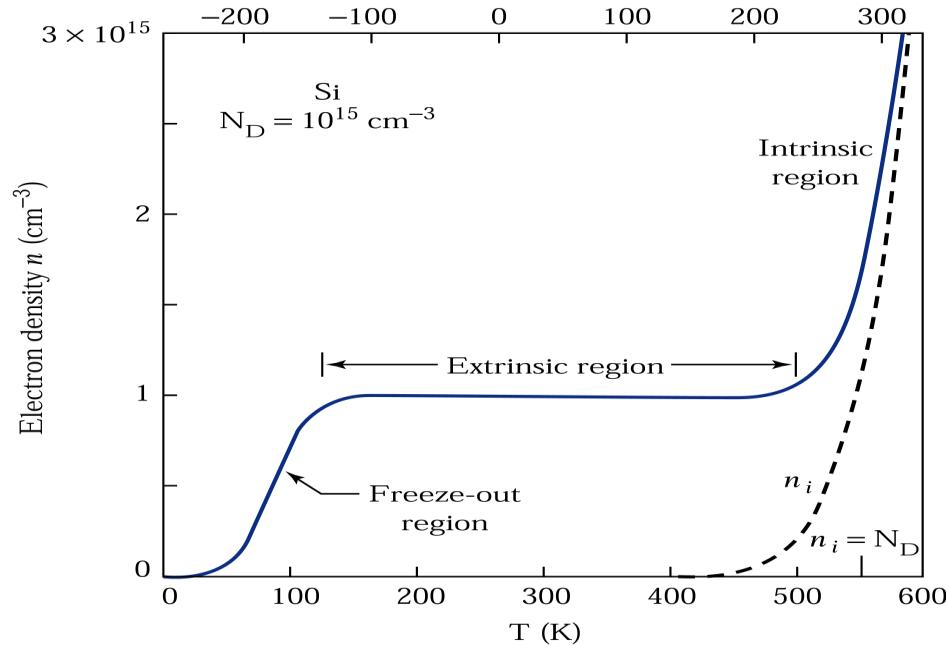
\includegraphics[width=0.9\textwidth]{figure/ch3掺杂硅在不同温度下的载流子浓度.png}
    \caption{掺杂硅在不同温度下的载流子浓度}
    \label{fig:ch3-doped-si-carrier-concentration}
\end{figure}

\begin{problem}
    \textbf{所用常数与已知量：}
    \[
    \begin{aligned}
        k_0&=8.617333262\times10^{-5}\ \mathrm{eV\cdot K^{-1}},
        \qquad E_g=0.67\ \mathrm{eV},\\
        N_c(300\ \mathrm{K})&=1.05\times10^{19}\ \mathrm{cm}^{-3},
        \qquad N_v(300\ \mathrm{K})=3.90\times10^{18}\ \mathrm{cm}^{-3},\\
        N_D&=5\times10^{15}\ \mathrm{cm}^{-3},
        \qquad N_A=2\times10^9\ \mathrm{cm}^{-3}.
    \end{aligned}
    \]
    按题意，两温度下均取上述$E_g$，并假定态密度有效质量不随温度变化。

    \textbf{题面：}利用题7所给的$N_c,N_v$及$E_g=0.67\ \mathrm{eV}$，
    求$300\ \mathrm{K}$和$500\ \mathrm{K}$时，含施主浓度
    $N_D=5\times10^{15}\ \mathrm{cm}^{-3}$、受主浓度
    $N_A=2\times10^9\ \mathrm{cm}^{-3}$的锗中电子及空穴浓度。
    $300\ \mathrm{K}$按强电离区计算，$500\ \mathrm{K}$按过渡区计算。

    \textbf{解析：}两个温区均视杂质完全电离，净施主浓度为
    \[
    \Delta N=N_D-N_A=4.999998\times10^{15}\ \mathrm{cm}^{-3}.
    \]
    有效态密度和本征浓度的计算式为
    \[
    N_{c,v}(T)=N_{c,v}(300)\left(\frac{T}{300}\right)^{3/2},
    \qquad n_i=\sqrt{N_cN_v}\exp\!\left(-\frac{E_g}{2k_0T}\right).
    \]
    \begin{center}
        \small
        \begin{tabular}{c c c c}
            \hline
            物理量 & 计算式 & $300\ \mathrm{K}$ & $500\ \mathrm{K}$ \\
            \hline
            温度因子 & $(T/300)^{3/2}$ & $1$ & $2.1517$ \\
            $N_c$ & $N_c(300)(T/300)^{3/2}$ & $1.05\times10^{19}$ & $2.26\times10^{19}$ \\
            $N_v$ & $N_v(300)(T/300)^{3/2}$ & $3.90\times10^{18}$ & $8.39\times10^{18}$ \\
            $k_0T\ (\mathrm{eV})$ & $8.617333262\times10^{-5}T$ & $0.02585$ & $0.04309$ \\
            $n_i$ & $\sqrt{N_cN_v}\exp[-E_g/(2k_0T)]$ & $1.51\times10^{13}$ & $5.78\times10^{15}$ \\
            \hline
        \end{tabular}
    \end{center}

    \textbf{（1）$300\ \mathrm{K}$：强电离区。}
    因$n_i\ll\Delta N$，可忽略少数载流子对电中性条件的贡献，
    取$n_0\simeq\Delta N$，再由$n_0p_0=n_i^2$求$p_0$。

    \textbf{（2）$500\ \mathrm{K}$：过渡区。}
    本征激发已不可忽略，需联立
    \[
    \begin{cases}
        n_0-p_0=\Delta N,\\
        n_0p_0=n_i^2,
    \end{cases}
    \quad\Longrightarrow\quad
    n_0=\frac{\Delta N+\sqrt{(\Delta N)^2+4n_i^2}}{2},
    \qquad p_0=\frac{n_i^2}{n_0}.
    \]
    两种温区的计算式与结果对照如下，浓度单位均为$\mathrm{cm}^{-3}$。
    \begin{center}
        \small
        \begin{tabular}{c c c}
            \hline
            物理量 & $300\ \mathrm{K}$（强电离区） & $500\ \mathrm{K}$（过渡区） \\
            \hline
            电子计算式 & $n_0\simeq\Delta N$ & $n_0=[\Delta N+\sqrt{(\Delta N)^2+4n_i^2}]/2$ \\
            电子浓度 & $\boxed{5.00\times10^{15}}$ & $\boxed{8.80\times10^{15}}$ \\
            空穴计算式 & $p_0=n_i^2/\Delta N$ & $p_0=n_i^2/n_0$ \\
            空穴浓度 & $\boxed{4.55\times10^{10}}$ & $\boxed{3.80\times10^{15}}$ \\
            \hline
        \end{tabular}
    \end{center}
\end{problem}

\begin{problem}
    \textbf{所用常数与已知量：}
    \[
    \begin{aligned}
        k_0&=8.617333262\times10^{-5}\ \mathrm{eV\cdot K^{-1}},\\
        N_D&=10^{15}\ \mathrm{cm}^{-3},\qquad N_A=0,\qquad g_D=2,\\
        N_c(300\ \mathrm{K})&=2.80\times10^{19}\ \mathrm{cm}^{-3},
        \qquad E_c-E_D=0.045\ \mathrm{eV}.
    \end{aligned}
    \]
    其中$N_c(300\ \mathrm{K})$及磷施主电离能为补充采用的常用参数，
    用于$77\ \mathrm{K}$的不完全电离计算；假定态密度有效质量不随温度变化。
    % 补充参数来源：华盛顿大学硅材料参数表及磷施主能级研究。
    % https://faculty.washington.edu/tcchen/EE527Wi/Notes/EE%20527%2001-15%202014.pdf
    % https://www.nature.com/articles/s41598-017-06296-8
    本征载流子浓度取给定近似值：
    \begin{center}
        \begin{tabular}{c c c c c}
            \hline
            $T\ (\mathrm{K})$ & $77$ & $300$ & $500$ & $800$ \\
            \hline
            $n_i\ (\mathrm{cm}^{-3})$ & $10^{-20}$ & $10^{10}$ & $2.2\times10^{14}$ & $10^{17}$ \\
            \hline
        \end{tabular}
    \end{center}

    \textbf{题面（13）：}有一块掺磷的N型硅，$N_D=10^{15}\ \mathrm{cm}^{-3}$，
    分别计算$77\ \mathrm{K}$、$300\ \mathrm{K}$、$500\ \mathrm{K}$、
    $800\ \mathrm{K}$时导带中的电子浓度，本征载流子浓度采用上述数值。

    \textbf{解析：}采用非简并近似，按温度分别处理杂质电离及本征激发。

    \textbf{（1）$77\ \mathrm{K}$：考虑杂质不完全电离。}
    本征激发可忽略，故$n_0\simeq n_D^+$。由
    \[
    n_0=N_c\exp\!\left(\frac{E_F-E_c}{k_0T}\right),\qquad
    n_D^+=\frac{N_D}{1+2\exp[(E_F-E_D)/(k_0T)]},
    \]
    消去$E_F$，令
    \[
    A=\frac{2}{N_c}\exp\!\left(\frac{E_c-E_D}{k_0T}\right),
    \quad An_0^2+n_0-N_D=0,
    \quad n_0=\frac{2N_D}{1+\sqrt{1+4AN_D}}.
    \]
    其中
    \[
    N_c(77)=2.80\times10^{19}\left(\frac{77}{300}\right)^{3/2}
    =3.64\times10^{18}\ \mathrm{cm}^{-3},\qquad
    A=4.84\times10^{-16}\ \mathrm{cm}^{3}.
    \]
    因而$n_0\simeq7.37\times10^{14}\ \mathrm{cm}^{-3}$，施主电离率约为$73.7\%$。

    \textbf{（2）较高温度：杂质近乎完全电离。}
    联立$n_0-p_0=N_D$与$n_0p_0=n_i^2$，得
    \[
    n_0=\frac{N_D+\sqrt{N_D^2+4n_i^2}}{2}.
    \]
    各温度下采用的算式和结果汇总如下，浓度单位均为$\mathrm{cm}^{-3}$。
    \begin{center}
        \small
        \begin{tabular}{c c c c}
            \hline
            $T\ (\mathrm{K})$ & 温区或处理方法 & 电子浓度计算式 & $n_0$ \\
            \hline
            $77$ & 不完全电离 & $2N_D/[1+\sqrt{1+4AN_D}]$ & $\boxed{7.37\times10^{14}}$ \\
            $300$ & 强电离区 & $n_0\simeq N_D$ & $\boxed{1.00\times10^{15}}$ \\
            $500$ & 计入本征激发 & $[N_D+\sqrt{N_D^2+4n_i^2}]/2$ & $\boxed{1.046\times10^{15}}$ \\
            $800$ & 本征激发占主导 & $[N_D+\sqrt{N_D^2+4n_i^2}]/2$ & $\boxed{1.005\times10^{17}}$ \\
            \hline
        \end{tabular}
    \end{center}
    $800\ \mathrm{K}$时$n_i\gg N_D$，也可近似取$n_0\simeq n_i=10^{17}\ \mathrm{cm}^{-3}$。
\end{problem}

\begin{problem}
    \textbf{所用常数与已知量：}
    \[
    \begin{aligned}
        k_0&=8.617333262\times10^{-5}\ \mathrm{eV\cdot K^{-1}},
        \qquad T=300\ \mathrm{K},\\
        N_D&=9\times10^{15}\ \mathrm{cm}^{-3},
        \qquad N_A=1.1\times10^{16}\ \mathrm{cm}^{-3},\\
        n_i&=10^{10}\ \mathrm{cm}^{-3}.
    \end{aligned}
    \]

    \textbf{题面（14）：}计算含施主浓度$N_D=9\times10^{15}\ \mathrm{cm}^{-3}$
    及受主浓度$N_A=1.1\times10^{16}\ \mathrm{cm}^{-3}$的硅，
    在$300\ \mathrm{K}$时的电子、空穴浓度以及费米能级的位置。
    已知此时$n_i=10^{10}\ \mathrm{cm}^{-3}$。

    \textbf{解析：}室温下杂质近乎完全电离，补偿后净受主浓度为
    \[
    \Delta N_A=N_A-N_D=2.00\times10^{15}\ \mathrm{cm}^{-3}>0,
    \]
    故材料为P型。由电中性条件$p_0-n_0=\Delta N_A$及$n_0p_0=n_i^2$，
    因$n_i\ll\Delta N_A$，可取$p_0\simeq\Delta N_A$。
    费米能级相对本征能级的位置由
    $E_F-E_i=-k_0T\ln(p_0/n_i)$确定。
    \begin{center}
        \begin{tabular}{c c c}
            \hline
            物理量 & 计算式 & 结果 \\
            \hline
            空穴浓度$p_0$ & $N_A-N_D$ & $\boxed{2.00\times10^{15}\ \mathrm{cm}^{-3}}$ \\
            电子浓度$n_0$ & $n_i^2/p_0$ & $\boxed{5.00\times10^4\ \mathrm{cm}^{-3}}$ \\
            $E_F-E_i$ & $-k_0T\ln(p_0/n_i)$ & $\boxed{-0.316\ \mathrm{eV}}$ \\
            \hline
        \end{tabular}
    \end{center}
    即费米能级位于本征能级$E_i$下方约$0.316\ \mathrm{eV}$。
\end{problem}

\begin{problem}
    \textbf{所用常数与已知量：}
    \[
    \begin{aligned}
        k_0&=8.617333262\times10^{-5}\ \mathrm{eV\cdot K^{-1}},\\
        N_A&=10^{22}\ \mathrm{m}^{-3}=10^{16}\ \mathrm{cm}^{-3},
        \qquad N_D=0,\\
        n_i(300\ \mathrm{K})&=10^{10}\ \mathrm{cm}^{-3},
        \qquad n_i(600\ \mathrm{K})=3\times10^{15}\ \mathrm{cm}^{-3}.
    \end{aligned}
    \]
    单位换算：$1\ \mathrm{m}^{-3}=10^{-6}\ \mathrm{cm}^{-3}$。

    \textbf{题面（15）：}掺有浓度为每立方米$10^{22}$个硼原子的硅材料，
    分别计算$300\ \mathrm{K}$、$600\ \mathrm{K}$时费米能级的位置以及多数、少数载流子浓度。
    本征载流子浓度分别取$10^{10}\ \mathrm{cm}^{-3}$、$3\times10^{15}\ \mathrm{cm}^{-3}$。

    \textbf{解析：}硼为受主，材料为P型，多数载流子为空穴，少数载流子为电子。
    两个温度下均视受主完全电离，联立
    \[
    \begin{cases}
        p_0-n_0=N_A,\\
        n_0p_0=n_i^2,
    \end{cases}
    \quad\Longrightarrow\quad
    p_0=\frac{N_A+\sqrt{N_A^2+4n_i^2}}{2},\qquad
    n_0=\frac{n_i^2}{p_0}.
    \]
    $300\ \mathrm{K}$时$n_i\ll N_A$，按强电离区取$p_0\simeq N_A$；
    $600\ \mathrm{K}$时需保留本征激发，按过渡区使用上述完整解。
    费米能级统一用$E_F-E_i=-k_0T\ln(p_0/n_i)$计算。
    \begin{center}
        \small
        \begin{tabular}{c c c c}
            \hline
            物理量 & 计算式 & $300\ \mathrm{K}$ & $600\ \mathrm{K}$ \\
            \hline
            $k_0T\ (\mathrm{eV})$ & $k_0T$ & $0.02585$ & $0.05170$ \\
            多子$p_0\ (\mathrm{cm}^{-3})$ & $[N_A+\sqrt{N_A^2+4n_i^2}]/2$ & $\boxed{1.00\times10^{16}}$ & $\boxed{1.083\times10^{16}}$ \\
            少子$n_0\ (\mathrm{cm}^{-3})$ & $n_i^2/p_0$ & $\boxed{1.00\times10^4}$ & $\boxed{8.31\times10^{14}}$ \\
            $E_F-E_i\ (\mathrm{eV})$ & $-k_0T\ln(p_0/n_i)$ & $\boxed{-0.357}$ & $\boxed{-0.0664}$ \\
            \hline
        \end{tabular}
    \end{center}
    升温后本征激发增强，少数载流子浓度明显增加，费米能级向$E_i$靠近。
\end{problem}
